%%%%%%%%%%%%%%%%%%%%%%%%%%%%%% -*- Mode: Latex -*- %%%%%%%%%%%%%%%%%%%%%%%%%%%%
%% uhtest-body.tex -- 
%% Author          : Robert Brewer
%% Created On      : Fri Oct  2 16:30:37 1998
%% Last Modified By: Robert Brewer
%% Last Modified On: Mon Oct  5 16:01:29 1998
%% RCS: $Id: uhtest-body.tex,v 1.1 1998/10/06 02:07:14 rbrewer Exp $
%%%%%%%%%%%%%%%%%%%%%%%%%%%%%%%%%%%%%%%%%%%%%%%%%%%%%%%%%%%%%%%%%%%%%%%%%%%%%%%
%%   Copyright (C) 1998 Robert Brewer
%%%%%%%%%%%%%%%%%%%%%%%%%%%%%%%%%%%%%%%%%%%%%%%%%%%%%%%%%%%%%%%%%%%%%%%%%%%%%%%
%% 

\chapter{Introduction}

Every dissertation should have an introduction.  You might not realize
it, but the introduction should introduce the concepts, background,
and goals of the dissertation.

Examples of great literature can be found in table \ref{tab:example-1}.

%% Here is an example of how to create a floating table. Note that the caption
%% occurs _before_ the table, unlike a figure where it appears after!
%%
%% The "[htbp]" allows the table to be placed: here, top of page, bottom of
%% page or on a seperate floats page, whatever works best.
\begin{table}[htbp]
  %% If you have a really long caption, you can enclose a short version for the
  %% the List of Tables in "[]", and the full caption in "{}" as we do here
  \caption[A normal size table.]{A normal size table. There has been a complaint
    that table captions are not single-spaced, but they should be. This is a
    test of that feature.}
  %% This label allows references from other parts of the text to be
  %% automatically calculated. Labels usually start with three letters
  %% describing what is being tabled followed by a colon. This prevents label
  %% mixups. Note that the label must follow the caption for proper numbering.
  \label{tab:example-1}
  \begin{center}
    \begin{tabular}{|l|r|}
      \hline 
      Title & Author \\
      \hline
      War And Peace & Leo Tolstoy \\
      The Great Gatsby & F. Scott Fitzgerald \\ \hline
    \end{tabular}
  \end{center}
\end{table}

\chapter{Previous Work}

Some other research was once performed. You can check out a beautiful picture
in figure \ref{fig:example-1}.

\begin{figure}[htbp]
  \centering
  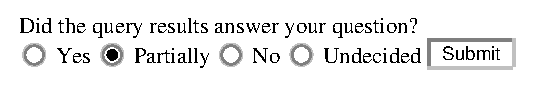
\includegraphics{example-figure.eps}
  \caption{An example of included Encapsulated PostScript (EPS).}
  \label{fig:example-1}
\end{figure}

\section{URLs}
In this modern age, you may find that you wish to include URLs or pathnames
which both tend to be long and hard for TeX to deal with because it doesn't
know where to insert linebreaks. The ``{\tt url}'' package (loaded in the main
uhtest.tex file) allows one to deal with these URLs. For example:

Here is an URL which cannot be broken, leading to terrible output
$<$http://www.hotwired.com/webmonkey/98/16/index2a.html$>$
%% The "<>" have to be entered in math mode, that's where the "$"s come from.

Using the package we get the much nicer \url{<http://www.hotwired.com/
webmonkey/98/16/index2a.html>} which LaTeX can handle just fine. Even better,
the parameter to {\tt $\backslash$url} can have spaces inserted anywhere so you
can make the LaTeX source lines in your text editor wrap nicely.

A few notes. It is recommended that you enclose your URLs in ``$<>$'' to ensure
that any punctuation around the URL won't be confused as part of the URL. You
can use URLs in your bibliography too (see the {\tt uhtest.bib} file for an
example). Finally, if you need to use a tilde in your URL then things are a
little trickier. One way to do it is like this:
\url{<http://www.dartmouth.edu/}$\sim$\url{jonh/ff-cache/1.html>}. The {\tt
$\backslash$url} style uses math mode internally, so we break the URL into two
pieces, and stick a tilde from math mode inbetween the two parts.

\section{Bibliography Citations}
Citing references to your bibliography is easy \cite{lamport:latex}
\cite{patashnik:bibtex}. First you build a BibTeX file which contains the
records for all of the works you wish to cite. This file ends with a ``{\tt
.bib}'' extension. Then in your body you use the ``{\tt $\backslash$cite}''
command with the label you gave to the record in question. The final steps are: 
run LaTeX once, run BibTeX, and then run LaTeX twice more. You should now have
a bibliography that includes those citations.

\chapter{Conclusion}

This is going to be the chapter where I check the length of the page to make
sure the bottom margin works out all right.  I hope you don't mind long
annoying and useless paragraphs because you are sure to get a lot of them here!

\section{Widgets}

This is going to be the chapter where I check the length of the page
to make sure the bottom margin works out all right.  I hope you don't
mind long annoying and useless paragraphs because you are sure to get
a lot of them here!

\subsection{Sub-Widgets}

This is going to be the chapter where I check the length of the page
to make sure the bottom margin works out all right.  I hope you don't
mind long annoying and useless paragraphs because you are sure to get
a lot of them here!

\subsubsection{Sub-Sub-Widgets}

This is going to be the chapter where I check the length of the page
to make sure the bottom margin works out all right.  I hope you don't
mind long annoying and useless paragraphs because you are sure to get
a lot of them here!

\paragraph{Para-Widgets}

This is going to be the chapter where I check the length of the page
to make sure the bottom margin works out all right.  I hope you don't
mind long annoying and useless paragraphs because you are sure to get
a lot of them here!

\subparagraph{Sub-Para-Widgets}

This is going to be the chapter where I check the length of the page
to make sure the bottom margin works out all right.  I hope you don't
mind long annoying and useless paragraphs because you are sure to get
a lot of them here!

This is going to be the chapter where I check the length of the page
to make sure the bottom margin works out all right.  I hope you don't
mind long annoying and useless paragraphs because you are sure to get
a lot of them here!

This is going to be the chapter where I check the length of the page
to make sure the bottom margin works out all right.  I hope you don't
mind long annoying and useless paragraphs because you are sure to get
a lot of them here!

This is going to be the chapter where I check the length of the page
to make sure the bottom margin works out all right.  I hope you don't
mind long annoying and useless paragraphs because you are sure to get
a lot of them here!

This is going to be the chapter where I check the length of the page
to make sure the bottom margin works out all right.  I hope you don't
mind long annoying and useless paragraphs because you are sure to get
a lot of them here!

This is going to be the chapter where I check the length of the page
to make sure the bottom margin works out all right.  I hope you don't
mind long annoying and useless paragraphs because you are sure to get
a lot of them here!

This is going to be the chapter where I check the length of the page
to make sure the bottom margin works out all right.  I hope you don't
mind long annoying and useless paragraphs because you are sure to get
a lot of them here!

This is going to be the chapter where I check the length of the page
to make sure the bottom margin works out all right.  I hope you don't
mind long annoying and useless paragraphs because you are sure to get
a lot of them here!

This is going to be the chapter where I check the length of the page
to make sure the bottom margin works out all right.  I hope you don't
mind long annoying and useless paragraphs because you are sure to get
a lot of them here!

This is going to be the chapter where I check the length of the page
to make sure the bottom margin works out all right.  I hope you don't
mind long annoying and useless paragraphs because you are sure to get
a lot of them here!

This is going to be the chapter where I check the length of the page
to make sure the bottom margin works out all right.  I hope you don't
mind long annoying and useless paragraphs because you are sure to get
a lot of them here!

This is going to be the chapter where I check the length of the page
to make sure the bottom margin works out all right.  I hope you don't
mind long annoying and useless paragraphs because you are sure to get
a lot of them here!

This is going to be the chapter where I check the length of the page
to make sure the bottom margin works out all right.  I hope you don't
mind long annoying and useless paragraphs because you are sure to get
a lot of them here!

This is going to be the chapter where I check the length of the page
to make sure the bottom margin works out all right.  I hope you don't
mind long annoying and useless paragraphs because you are sure to get
a lot of them here!

This is going to be the chapter where I check the length of the page
to make sure the bottom margin works out all right.  I hope you don't
mind long annoying and useless paragraphs because you are sure to get
a lot of them here!

This is going to be the chapter where I check the length of the page
to make sure the bottom margin works out all right.  I hope you don't
mind long annoying and useless paragraphs because you are sure to get
a lot of them here!
